\chapter{FLB框架的应用}\label{chapter:FLBDTW}

本章主要介绍如何使用FLB框架处理基于动态时间卷曲距离的查询。首先,章节\ref{sec-c5-DTWsummary}介绍了利用包围信封为DTW距离提供概要数据。 然后,章节\ref{sec-c5-lowerBound}介绍了基于包围信封的DTW距离下界。其次,章节\ref{sec-c5-algorithm}介绍了算法DTW-FLB,以处理当使用动态时间卷曲距离作为距离度量准则时的查询。接着,章节\ref{sec-c5-algorithm}展示了DTW-FLB算法的有效性和可扩展性。再其次,章节 \ref{sec-c5-conclusion}小结本章的研究内容。最后,本章涉及到的证明内容放在附件部分。


\section{基于动态时间卷曲距离的概要数据}\label{sec-c5-DTWsummary}

\subsection{基于动态时间卷曲距离的轨迹相似度度量}\label{sec-c5-DTW}
\begin{figure}[t]
	\centering
	\includegraphics[width=0.48\textwidth]{Fig/chapter5/DTW}
	\caption{带约束的动态时间卷曲}
	\label{fig:DTW}
\end{figure}
给定查询轨迹$\cal Q$表示为${\cal Q}=\{\vq_{0}, \vq_{1}, \cdots, \vq_{n-1}\}$,以及一条候选轨迹$\cal C$表示为${\cal C}=\{\vc_{0}, \vc_{1}, \cdots, \vc_{n-1}\}$,其中$n$为轨迹长度,每个轨迹点来自$d$维空间,即$\vq_{i},\vc_{i} \in R^{d}$。为使用动态时间卷曲距离匹配 $\cal Q$和$\cal C$,我们构建了一个$n\times n$的代价矩阵$cost$。其中第$i$行第$j$列的元素记录了使用欧式距离匹配$\vq_{i}$和$\vc_{j}$两点之间的代价。动态时间卷曲距离的目的就是发现一条从如图\ref{fig:DTW}所示左下角出发到右上角结束的代价最小的路线/卷曲路径。一条卷曲路径需满足如下3个特别的约束:
\begin{itemize}
	\item \textbf{边界条件}: 路径从代价矩阵的$[0,0]$号格子出发并在$[n-1,n-1]$号格子结束。
	
	\item \textbf{连续性}: 如果路径中相邻的两次权重值分别取自代价矩阵的$[i,j]$ 和 $[i^{'},j^{'}]$两个单元,那么这两个单元的位置关系必满足如下条件:$i^{'}-i\le 1$ 和 $j^{'} - j \le 1$。这个约束使得路径在扩展过程中只能从一个格子扩展到其半径为1周边的格子。
	\item \textbf{单调性}: 如果路径中相邻的两次权重值分别取自代价矩阵的$[i,j]$ 和 $[i^{'},j^{'}]$两个单元,那么这两个单元的位置关系还须满足如下条件: $i^{'}-i\ge 0$ 和 $j^{'} - j \ge 0$。这个约束使得路径搜索过程中只能前进不能后退。
\end{itemize}
根据以上描述,我们形式化给出动态时间卷曲距离的定义:
\begin{eqnarray}\label{eq:dtwDef}
DTW({\cal Q}, {\cal C})= \min{\sum\nolimits_{k=1}^{K}\vw_{k}} \qquad {(n\le K < 2n)}
\end{eqnarray}
其中,$\vw_{k}$是卷曲路径$\cal W$的第$k$个元素,其值来源于代价矩阵的第$[i,j]$个格子。
$\cal{W}=\{$ $\vw_{1}$$,\vw_{2}$$,\cdots,\vw_{K}\}$, 代表了一条匹配$\cal{Q}$ 和 $\cal{C}$卷曲路径。

动态时间卷曲距离的计算过程可通过动态规划算法实现,因为其计算过程可以看作如下最优子结构的递归:
\begin{eqnarray}\label{eq:dtwdef}
DTW&=&\gamma(n-1,n-1) \\ \nonumber
\gamma(i,j)&=&SED(\vq_{i}, \vc_{j}) + \min(\gamma(i-1,j-1), \gamma(i-1,j), \nonumber \\
&&\gamma(i,j-1))  \quad s.t.  \quad |i-j| \le \delta
\end{eqnarray}
其中$\delta$ 是一个全局约束,用于限制查询路径的可以偏离对角线的范围。图\ref{fig:DTW}中显示了当$\delta=4$时,灰色部分即为卷曲路径的查询范围。
使用全局约束的原因有两个:(i)该约束可以提高查询的效率,$\delta$使得动态时间卷曲距离的计算复杂度由原来的$n^2$降低为$\frac{n^2}{\delta}$。
(ii)该约束还能有效抑制无效的卷曲路径的产生。比如,一轨迹的一小段匹配到另一轨迹的一大段上情况。


\subsection{基于包围信封的概要数据}\label{sec-c5-BE}
\begin{figure}[t]
	\centering
	\includegraphics[width=0.48\textwidth]{Fig/chapter5/BE}
	\caption{包围信封}
	\label{fig:BE}
\end{figure}
包围信封(Bounding Envelope,BE)概念来源于时间序列数据分析,其目的是使用一上一下两条边界曲线来包住给定的时间序列。如图\ref{fig:BE}所示,红色虚线为一条时间序列,$U$和$L$两条线分别代表了这条时间序列的上界和下界。给定时间序列,构造其包围信封的方法有许多。由于本文的目的是利用包围信封构造概要数据,故所构造的包围信封包含的数据量要低。此外,所构造的包围信封还应具有多粒度特性,以适应FLB框架的需求。

为此,引入基于时间序列划分(Time Series Segmentation)的包围信封。其做法是给定一条时间序列$\cal S$,将其均匀划分成多个等长度的片段。我们使用$s_{l}^{p}= {[lb, ub, len]}$来表示其中一条片段$\{\vq_{i}, \vq_{i+1}, \cdots, \vq_{j} \}$的最小包围盒(Minimum Bounding Rectangle, MBR)。其中$l$代表划分的粒度(粒度越细,每个片段的长度越短),$p$代表该片段在当前划分下所对应的位置。$lb$ 和 $ub$分别代表该片段的最小值和最大值,$len$代表该片段的长度。由$\{s_{l}^{1}, \cdots s_{l}^{n'}\}$所构成的列表代表了该次划分所对应的包围信封,其用${\cal S}_{l}$表示。在第0层,整个时间序列被看做一个划分,接着将其均匀切成$R$个不相交的相连子片段。这个过程可以一直持续下去,直到每个片段的长度为1截止。

\begin{table}[t]
	\centering  
	\renewcommand\arraystretch{1.2}
	\begin{tabular}{|c|c|c|c|c|c|c|c|c|} 
		\hline
		${\cal S}_{0}$ &  \multicolumn{4}{|c|}{$s_{0}^{0}={[2,5,4]}$} \\ \hline
		${\cal S}_{1}$ & \multicolumn{2}{|c|}{$s_{1}^{0}={[2,5,2]}$} & \multicolumn{2}{|c|}{$s_{1}^{1}={[3,4,2]}$} \\ \hline 
		${\cal S}_{2}$ & \multicolumn{1}{|c|}{$s_{2}^{0}={[5,5,1]}$} & \multicolumn{1}{|c|}{$s_{2}^{1}={[2,2,1]}$} &
		\multicolumn{1}{|c|}{$s_{2}^{2}={[4,4,1]}$} &  \multicolumn{1}{|c|}{$s_{2}^{3}={[3,3,1]}$} \\ \hline 
		$Q$ & 5 & 2 & 4 & 3
		\\ \hline
	\end{tabular}
	\caption{时间序列$\cal S$的多粒度包围盒}
	\label{table:BE}
\end{table}
表格\ref{table:BE}介绍了给定时间序列${\cal S}=\{5,2,4,3\}$,计算其不同粒度包围盒的过程。其中,$R$的值设置为2。即从粗粒度到细粒度切分的过程中,每次将一个片段均匀划分成2个子片段。不失一般性,接下来的示例和实验室中,我们都将$R$的值设置为2。值得注意的是,本文采用的划分为均匀划分,而相关文章中所提非均匀划分的方法也可以被使用。此外,由于是均匀划分,我们可以推算出每个片段的长度,故其值无需保存。
 

%
%为适应动态时间卷曲计算和FLB所要求的概要数据具有多粒特性这两个需求,本文首先使用如下方法为给定的查询轨迹 $\cal Q$构造包围信封。
%\begin{eqnarray}\label{eq:dtwUL}
%{\cal U} = \{\vu_{0},\vu_{1},\cdots, \vu_{n-1} \} &,& \forall j  \, \vu_{i}^{j}=\max(\vq_{i-\delta}^{j} : \vq_{i+\delta}^{j}) \nonumber \\
%{\cal L} = \{\vl_{0},\vl_{1},\cdots, \vl_{n-1} \}&,& \forall j  \, \vl_{i}^{j}=\min(\vq_{i-\delta}^{j} : \vq_{i+\delta}^{j})
%\end{eqnarray}
%其中${\cal U}$ 和 ${\cal L}$分别对应了轨迹的上边界和下边界,$\delta$是动态时间卷曲距离计算中的全局约束。接下来,我们设计了基于$\cal U$和$\cal L$的多粒度包围信封。
%
%Here, ${\cal U}$ and ${\cal L}$ are the sequences of  upper and lower boundaries, and $\delta$ is the warping constraint of DTW.  Next, we design different degrees of approximation for the bounding envelope in Eq.  \ref{eq:hatUL}. 


\section{动态时间卷曲距离的下界}\label{sec-c5-lowerBound}
 本节将介绍如何根据包围信封计算动态时间卷曲距离的下界。首先将介绍点的上、下界,然后再介绍如何利用点的范围计算轨迹的下界。
 
\subsection{满足DTW约束的包围信封及下界} 
令 $\vq$ 和 $\vc$ 表示两个来自$d$维实数空间的点, 其中$\vc$的值已知,$\vq$的值不知道,但知道其在一个$d$维矩形$\{\vu, \vl\}$里,即$\forall j\in [0, d),  \,\, {\vl}^{j}  \le \vq^{j} \le \vu^{j}$。对$\vq$ 和 $\vc$之间的实际欧式距离我们无法计算出来,但可以通过如下引理计算出距离的下界。
\begin{lemma}\label{theory:SEDLB}
	给定 $\bq$ 、$\bc$ 以及$\bq$的包围矩形$\{\bu, \bl\}$,我们有
	$SED\_LB(\{{\bu},\bl \},\bc)\le SED(\bq,\bc)$, 其中 $SED\_LB(\{{\bu},\bl \},\bc)$ 的计算过程如下:
	\allowdisplaybreaks
	\begin{equation}
	SED\_LB(\{{\bu},\bl \},\bc) =
	\sum_{j=0}^{d-1} \begin{cases}
	({\bc}^{j}- {\bu}^{j})^2 & \emph{if} \,\,\,   \bu^{j} \le {\bc}^{j},\\
	\quad 0 &   \emph{if} \,\,\,  \bl^{j} \le  {\bc}^{j} \le \bu^{j},\\
	({\bl}^{j} -{\bc}^{j})^2 & \emph{if} \,\,\,    {\bc}^{j} \le \bl^{j}.\\
	\end{cases}
	\end{equation}
	\allowdisplaybreaks[4]
\end{lemma}

接着介绍如何构建满足动态时间卷曲距离的包围信封。根据包围信封的介绍,我们知道给定查询轨迹$\cal Q$,构建包围信封的最重要就是构造轨迹的上、下边界。同时,考虑到动态时间卷曲距离的全局约束特性。我们使用如下方法构建轨迹的上、下边界:
We next introduce how to construct a bounding envelope $\{{\cal U},{\cal L}\}$ for trajectory $\cal Q$, as defined below. %In Eq. \ref{eq:dtwUL},  ${\cal U}$ and 
\begin{eqnarray}\label{eq:dtwUL}
{\cal U} = \{\vu_{0},\vu_{1},\cdots, \vu_{n-1} \} &,& \forall j  \, \vu_{i}^{j}=\max(\vq_{i-\delta}^{j} : \vq_{i+\delta}^{j}) \nonumber \\
{\cal L} = \{\vl_{0},\vl_{1},\cdots, \vl_{n-1} \}&,& \forall j  \, \vl_{i}^{j}=\min(\vq_{i-\delta}^{j} : \vq_{i+\delta}^{j})
\end{eqnarray}
公式\ref{eq:dtwUL}中,${\cal U}$ 和 ${\cal L}$分别代表轨迹的上边界和下边界, $\delta$ 为动态时间卷曲距离中的全局约束。根据如上方式计算出来的包围盒,我们称之为满足动态时间卷曲约束的包围信封(Dynamic Time Warping constraint Bounding Envelope,DTWBE)。
此时,根据DTWBE$\{{\cal U}, {\cal L}\}  $和$\cal C$,我们可以给出如下距离定义:
\begin{equation}\label{eq:LBKeogh}
LB\_Keogh({\{\cal U,\cal L\},{\cal C}})=  \sum\nolimits_{i=0}^{n-1}	SED\_LB(\{{\vu_{i}},\vl_{i} \},\vc_{i})
\end{equation}
该定义可以看做是原始一维的$LB\_Keogh$下界在多维情况下的扩展,并得到如下下界定理:
\begin{theorem}\label{theorem:DTWLBK}
	给定轨迹$C$和待查询轨迹$Q$满足动态时间卷曲约束的包围信封$\{{\cal U}, {\cal L}\}$,我们有如下结论: $LB\_Keogh({\{\cal U,\cal L\},{\cal C}}) \le DTW(Q,C)$。
\end{theorem}


\subsection{基于多粒度包围信封的下界} 
为计算上一小节介绍的$LB\_Keogh$下界,需要传递DTWBE,其数据量为$2*n$。因此,不满足我们降低通信的目标。为此,本文首先设计了基于DTWBE的多粒度包围信封。多粒度信封的第$l$层边界计算方式如下:
%Let $\{\hat{{\cal U}}_l, \hat{{\cal L}}_l\}$ denote the level-$l$ approximation of boundaries ${\cal U}$ and ${\cal L}$ respectively. 
\begin{eqnarray}\label{eq:hatUL}
\hat{{\cal U}}_l =\{ \hat{\vu}_{l,0}, \hat{\vu}_{l,1},\cdots, \hat{\vu}_{l,2^l-1}\}  &,&
\forall j  \, \hat{\vu}_{l,i}^{j}=\max(\vu_{i\cdot 2^{L-l}}^{j} : \vu_{(i+1)\cdot 2^{L-l}-1}^{j})  \nonumber \\
\hat{{\cal L}}_l=\{\hat{\vl}_{l,0}, \hat{\vl}_{l,1},\cdots, \hat{\vl}_{l,2^l-1}\}   &,&
\forall j  \, \hat{\vl}_{l,i}^{j}=\min(\vl_{i\cdot 2^{L-l}}^{j} : \vl_{(i+1)\cdot 2^{L-l}-1}^{j})
\end{eqnarray}	
第$l$层的包围信封计算过程可看作将原来的DTWBE均匀切分成$2^l$块,然后对每个信封块计算仅使用两个$d$维点来构成新的包围信封。根据对公式 \ref{eq:hatUL}的观察,我们得到两种结论:(i)第$l$层的包围信封$\{\hat{{\cal U}}_{l}, \hat{{\cal L}}_{l}\}$ 数据量是第$l-1$层的两倍;(ii)第$l-1$层的数据被第$l$层包含。因此,在由粗到细发送包围信封这一概要数据时,除第$0$层外,其他层只需要发送一半的信息量(这一半数据的每个值需要用0和1标注其位置是在左边还是右边,但位置信息消耗的开销较小可忽略)。
那么假定远程结点已获取到查询轨迹$\cal Q$的第$l$层包围信封$\{\hat{{\cal U}}_l,\hat{{\cal L}}_l\}$,我们可通过如下公式来计算给定的候选与$\cal Q$的下界。
\begin{theorem}\label{theo:HPAA}
	给定轨迹$\cal Q$的第$l$层包围信封$\{\hat{{\cal U}}_{l}, \hat{{\cal L}}_{l}\}$和候选轨迹$\cal C$,我们得到如下结论:
	 $LB\_HPAA({  \{\hat{{\cal U}_{l}}, \hat{{\cal L}_{l}}\},\overline{{\cal C}}_{l}}) \le DTW(\cal Q, \cal C)$。其中$LB\_HPAA$的计算公式如下:
	 \begin{eqnarray}\label{bound:HPAA}
	 LB\_HPAA({\{\hat{{\cal U}_{l}}, \hat{{\cal L}_{l}}\},\overline{{\cal C}}_{l}})= 2^{L-l} \cdot \sum_{i=0}^{2^{l}-1} SED\_LB(\{ \hat{\bu}_{l,i}, \hat{\bl}_{l,i} \}, \bar{\bc}_{l,i})\nonumber
	 \end{eqnarray}
\end{theorem}
以上定理说明了给定查询轨迹的第$l$层包围信封和候选误轨迹差树的第$l$层均值,就能为原始轨迹和候选轨迹计算出动态时间卷曲距离的下界。同时该下界的计算复杂度是线性的,远小于距离本身二次的复杂度。因此,通过计算下界可为剪枝候选提供帮助。

此外,为配合FLB框架,我们需要证明,$LB\_HPAA$能随着粒度的增加而逐渐变紧。为此我们给出如下定理:
\begin{theorem}\label{theo:DTWLbInc}
	$LB\_HPAA$下界能随着查询轨迹包围信封层次的增加而逐渐变紧。
	也就是说: $LB\_HPAA({  \{\hat{{\cal U}_{l}}, \hat{{\cal L}_{l}}\},\overline{{\cal C}}_{l}})\le  LB\_HPAA({  \{\hat{{\cal U}}_{l+1}, \hat{\cal L}_{l+1}\},\overline{\cal C}_{l+1}})$。
\end{theorem}

%\textbf{是否可以构造上界?}
%至此为止,我们已经构造出了动态时间卷曲距离的下界。我们通过上一章知道如果能同时获取上界 尝试通过相同的概要数据计算出上界。


\section{基于动态时间距离的查询算法:DTW-FLB}\label{sec-c5-algorithm}
\subsection{DTW-FLB算法实现}
在上一节,我们已经利用多粒度概要数据得到越来越紧的动态时间卷曲距离下界。这使得在FLB框架中插入欧式距离成为可能。本节将详细介绍动态时间卷曲距离跟FLB相结合的查询算法DTW-FLB。DTW-FLB维持了FLB框架的主要结构,只对本章第一节所介绍的接口进行了具体实现。

\begin{algorithm}[t]
	\renewcommand{\baselinestretch}{1}
	\caption{{\sl DTW-FLB在协调者节点} \label{alg:DTWCor}}
	\begin{algorithmic}[2]
		\STATE /* \emph{DTW-FLB协调者结点函数接口实现} */
	\end{algorithmic}
	\textbf{coordinatorInit}(${\cal Q}, {\cal R}$)
	\begin{algorithmic}[1]
		\STATE 根据公式\ref{eq:dtwUL}构建DTWBE $\{{\cal U},{\cal L}\}$;
		 \FOR{$i=1$,$i<\log_{2}n$;$i++$}
			 \STATE 根据公式\ref{eq:hatUL}构建第$i$层包围信封 $ \{\hat{{\cal U}_{l}}, \hat{{\cal L}_{l}}\}$;
		\ENDFOR 
		\STATE $l\leftarrow -1$;
	\end{algorithmic}
	\textbf{generateInfo()}
	\begin{algorithmic}[1]
		\STATE $l\leftarrow l+1$; 
		\STATE \textbf{return} $ \{\hat{{\cal U}_{l}}, \hat{{\cal L}_{l}}\}$;
	\end{algorithmic}
\end{algorithm}

\begin{algorithm}[t]
	\renewcommand{\baselinestretch}{1}
	\caption{{\sl DTW-FLB在远程结点} \label{alg:DTWRemote}}
	\begin{algorithmic}[2]
		\STATE /* \emph{DTW-FLB远程结点函数接口实现} */
	\end{algorithmic}
	\textbf{remoteInit($TS_{r} , S_{r}$)}
	\begin{algorithmic}[1]
		\IF{第一次接受查询}
			\STATE 构建R-Tree索引。
			\FORALL{ $\cal C$ in $TS_{r}$}
				\STATE $\overline{\cal C} \leftarrow$  $\cal C$的均值序列; \COMMENT{候选轨迹获取所有层的均值构成的序列}
			\ENDFOR 
		\ENDIF
		\FORALL{ $\cal C$ in $TS_{r}$}
		\STATE $C\_BF \leftarrow 0$;  \COMMENT {为$\cal C$初始化下界}
		\STATE $S_{r}=S_{r} \cup C\_BF$;
		\ENDFOR
	\end{algorithmic}
	%(line \ref{a3:info} in Alg. \ref{alg:F2Co})
	\textbf{updateBounds}($S_{r}$, $m$) \qquad  $/*m=\{ \hat{\vu}_{l,i}, \hat{\vl}_{l,i} \}*/$
	\begin{algorithmic}[1]
		\IF{$l==0$}
			\STATE 使用索引树进行剪枝。
		\ENDIF
		\FORALL{ $\cal C$ in $TS_{r}$}
			\STATE $factor =2^{L-l}$;
			\STATE $c.lb=0$;
			 \FOR{$i=0$,$i<2^{l}$;$i++$}
					\STATE $p\_lb=SED\_LB(\{ \hat{\vu}_{l,i}, \hat{\vl}_{l,i} \}, \bar{\vc}_{l,i})$;
					\STATE $c.lb+=p\_lb$;
					\IF{$c.lb>\theta$}
						\STATE 将该轨迹从$S_{r}$中移除;
					\ENDIF
			\ENDFOR 
			\STATE 将$\cal C$的下界更新为$c.lb$;
		\ENDFOR
	\end{algorithmic}
\end{algorithm}
我们首先介绍如何实现那些运行在协调者节点的上的函数。在\textsf{coordinatorInit}函数中,我们首先对待查询轨迹计算出对应的DTWBE,接着基于DTWBE,我们构造多粒度的包围信封(即概要数据)。
由于FLB框架也是迭代式由粗到细的通信计算框架,在每轮的迭代中会将某一层的概要数据(包围信封)发送给远程结点。因此,在初始化过程中我们用$l$来记录当前已经发送到哪一层的数据,并将$l$初始化为$-1$,以便从第0层开始发送。此外,我们在\textsf{generateInfo}中准备将要发送的下一层概要数据,以便协调者结点发送。在发送数据时需要注意的是,由于$ \{\hat{{\cal U}_{l}}, \hat{{\cal L}_{l}}\}$的一半数据量已经包含在 $\{\hat{{\cal U}}_{l-1}, \hat{{\cal L}}_{l-1}\}$中,我们只需传输剩下的一半数据。


接着,介绍运行在远程结点的函数。对于\textsf{RemoteInit}函数,若远程结点是第一次接受查询,则会为每条候选轨迹进行哈尔小波变换。若不是,则为该结点所包含的每条轨迹初始化界特征信息(下界初始化为0,不记录上界)。在查询执行过程中\textsf{UpdateBounds}函数为候选更新下界。直接实现方式为根据下界的计算公式直接算出该值。但由于查询过程中的主要计算开销就是对所有候选更新界特征。因此,降低该过程的计算开销很有必要。
为降低更新界特征的计算开销,与上一章一样采用在更新界过程中进行剪枝的思想。根据$LB\_HPAA$的定义,我们可知该下界是一系列点距离下界的累加和。由于每个点距离下界都是大于0的数,因此我们可以在累加的过程中,通过判断当前已经累加的值是否已经超过剪枝的阈值。若超过了 则可提前将该值过滤掉。

除了以上步骤外,我们引入了R-tree来对轨迹构建索引以提高查询效率。具体地:首先,每个远程结点对自己局部轨迹数据构建R-tree索引。接着,当该结点第$0$层包围信封时,使用R-tree来剪枝。剪枝具体过程入下:(i) 遍历R-tree,找到跟查询轨迹包围信封相交的叶子节点。(ii)遍历这些叶子节点所包含的轨迹,并将这些轨迹列为候选。


 \subsection{DTW-FLB算法性能分析}
 本章节将从时间复杂度和空间复杂度量方面 对DTW-FLB进行性能分析。在此之前,我们仍使用$|C_{i}|$ 和 $|CS_{i}|$ 分别表示第$i$($i\ge 0$)次迭代前候选轨迹的数量和包含候选轨迹的远程结点数量,并假定迭代次数为$\lambda$($\lambda \le \log_{2}n$)。由于仅使用下界进行剪枝,因此存在着当概要数据发送完毕后,仍然存在着超过$k$个候选的情况。此时,我们使用$N'$来表示迭代计算结束后剩余候选的个数。
 
 \textbf{时间复杂度:}
 不考虑系统初始化时对所有候选进行哈尔小波变换的时间开销,DTW-FLB算法的时间主要来自两个方面:(i)算法3第2阶段的迭代更新的时间;(ii)对迭代结束后的候选计算真实动态时间卷曲距离的时间。第一方面的时间复杂度为$ \sum_{i=0}^{\lambda}d\cdot |C_{i}| \cdot 2^{i} $,该值与算法ED-FTB的迭代计算复杂度相同。第二方面的计算复杂度为$O(d \cdot \delta \cdot  N' \cdot n^2)$。因此,总的时间复杂度为$O(d \cdot ( \sum_{i=0}^{\lambda}  |C_{i}| \cdot 2^{i}+\delta  \cdot N' \cdot n^2))$。
 
 \textbf{通信复杂度:}
DTW-FLB算法的通信开销跟时间开销一样也是来自迭代发送包围信封和迭代结束后发送轨迹计算真实距离两个阶段。在迭代式发送包围阶段,第$i$次迭代中,协调者需要将第$i$层包围信封发送到候选结点中。由于,第$i$层包围信封已经有一半数据存在于第$i-1$层包围信封中且已被候选结点接受。因此,发送的数据量为$O(d\cdot 2^{i} \cdot |CS_{i}|)$。远程结点在接受到包围信封后,便更新下界并将局部最小的$k$个下界发送给协调者结点。这一过程发送的数据量最多为$O(|C_{i}|)$。总的来说,迭代过程中产生的通信开销为。假设迭代结束后,所剩$N'$($N'>k$)个结点分布在$m'$个远程结点中。此时最多需要将原始轨迹发送到$m'$个结点中。其所对应的开销为$O(d\cdot n\cdot m')$。结合这两个阶段,DTW-FLB的总通信开销为$O(\sum_{i=0}^{\log_{2}n}(d\cdot 2^{i} \cdot |CS_{i}| + |C_{i}|)+d\cdot n\cdot m'))$。

通过以上对DTW-FLB的分析,我们可以发现该算法对迭代剪枝的效果十分敏感。即剪枝结束后所剩候选的个数即包含这些候选的节点的个数,会严重影响到计算时间和通信开销。由于,DTW-FLB会在每一轮迭代中都会通过对部分候选轨迹计算真实的DTW距离用以更新全局过滤的阈值。该方法能保证该过滤阈值会不断逼近真实的第$k$小距离,因此最终会取得较好的剪枝效果。
 
 
 
  \section{实验分析}\label{sec-c5-Exp}
  \subsection{实验设置}
  本章工作在实验中使用北京出租车数据集,该数据集已被广泛应用于轨迹数据分析。该数据集采集了北京市三万多辆出租车在2013年10月份到12月份三个月内的行驶GPS轨迹。每个GPS轨迹点包含的数据维度较多,我们仅选取了位置(经度和纬度)、时间、速度和角度这五个维度的值,并进行了归一化预处理。我们从该数据集中截取了两个子数据集:\emph{T-Small}和\emph{T-Big}以分别验证算法的有效性和可扩展性。
  \emph{T-Small}截取了10月1至7号间 上午8点到10点的轨迹数据,并从中选出最长的1万条轨迹进行分析。
  \emph{T-Big} 截取了11月1号至12月31号间每天上午8至10点和下午5至7点两个时间段的1百万条轨迹数据。为满足实验需求,这两个数据集的每条轨迹长度均超过4,096。
  
  在本章的实验中,DTW-FLB算法使用JAVA实现。需要注意的是,在我们介绍中$\delta$的取值为整数来表示约束的范围。但为适应不同长度轨迹的需求,我们在实验中使用轨迹长度的百分比来表示约束范围。
  实验运行在一个包含12个结点的Spark集群上。每个结点包含8核因特尔E5335 2.0 GHz中央处理器和16GB的内存。
  
  \subsection{算法有效性} 
  \begin{figure}
  	\centering
  		\centering
  		\subfigure[$n=1,024$]{  
  			\label{fig:prune1024}
  			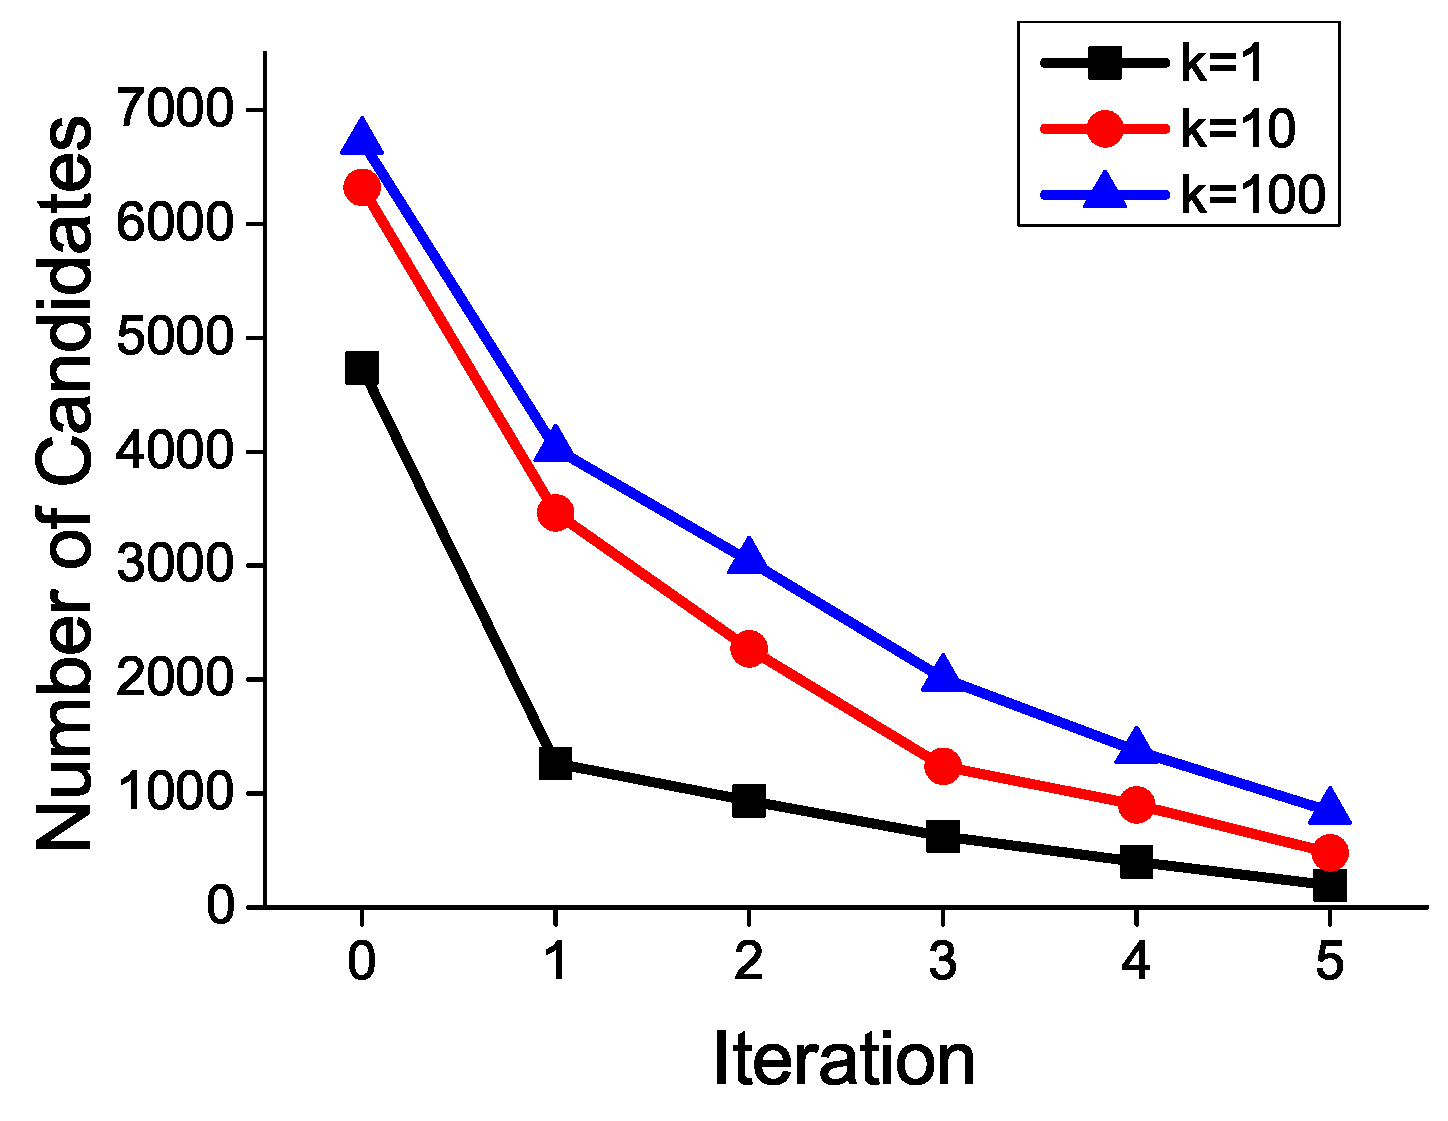
\includegraphics[width=1.78in]{Fig/chapter5/G1024.eps}
  		}
  		\subfigure[$n=2,048$]{
  			\label{fig:prune2048}
  			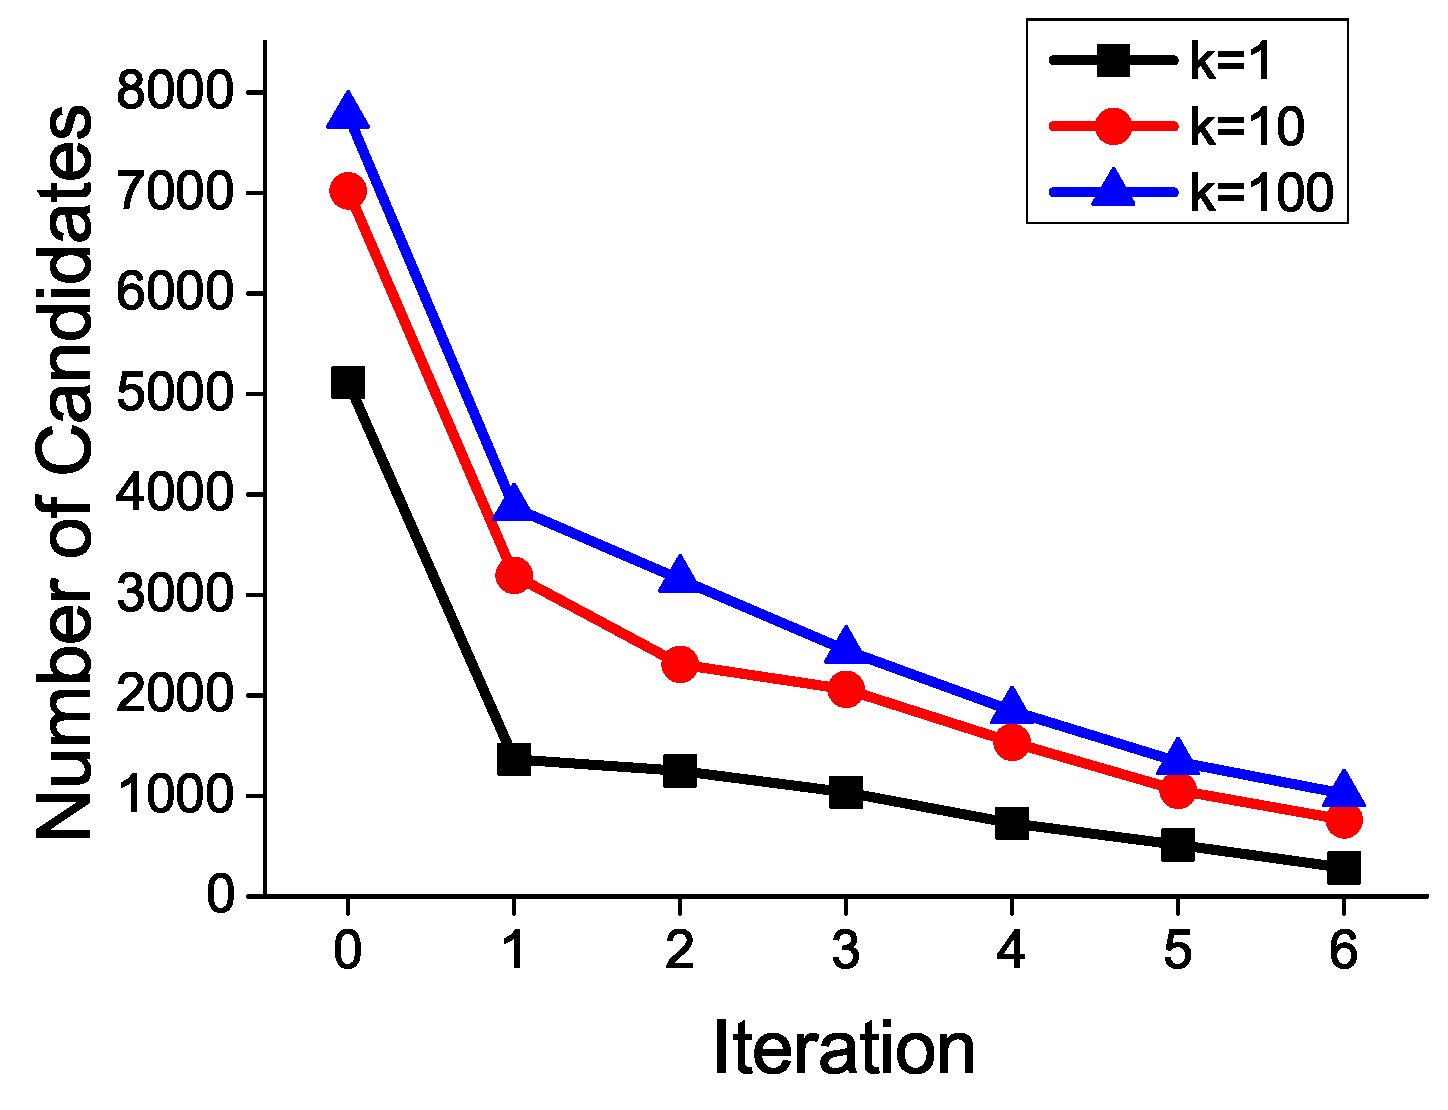
\includegraphics[width=1.78in]{Fig/chapter5/G2048.eps}
  		}
  		\subfigure[$n=4,096$]{
  			\label{fig:prune4096}
  			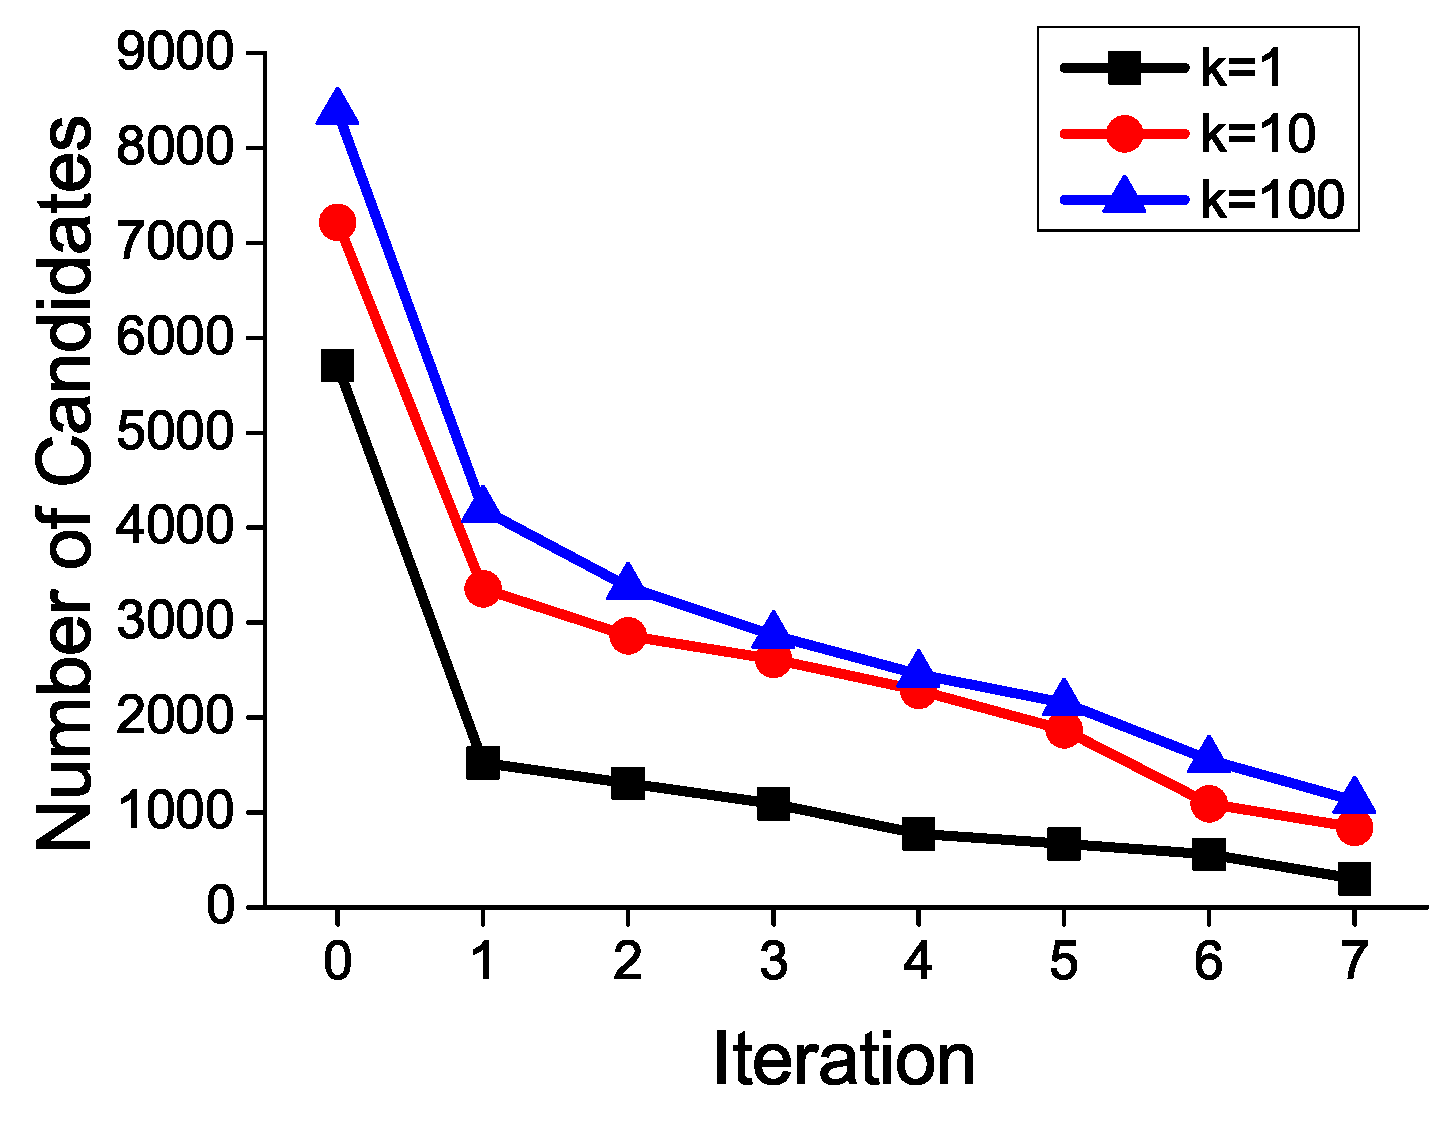
\includegraphics[width=1.78in]{Fig/chapter5/G4096.eps}
  		}
  		\caption{DTW-FLB剪枝效果}
  		\label{fig:hpaaPruning}
  \end{figure}


  首先,我们通过汇报迭代过程中每轮结束后所剩的候选的个数以展示DTW-FLB的剪枝效果。在该组实验中,我们设置轨迹长度$n$从256变化到4,096,$k$的值从1变化到100。图\ref{fig:hpaaPruning}展示了随着$k$和$n$变化后的剪枝的效果。从该图中我们可以看出在最开始的两轮迭代中,候选的个数急剧下降。此外,两轮迭代后所剩候选数较少。这说明,即使使用粗粒度的概要数据索引和剪枝策略的混合使用能起到较好的剪枝效果。在接下来的迭代中,我们可以发现候选个数降低比较平缓。由此可见,本文提出的由粗到细使用多粒度概要数据进行剪枝的思想具有较高的优越性,即它能够使用较少的数据剪枝掉大多数候选,从而达到了降低通信开销的目的。
  此外,可以发现随着$k$值的降低,我们能取得更好的剪枝效果。究其原因,$k$值较小时,所选取的全局过滤阈值随之降低即更接近真实的第$k$小真实距离值。
  
  \begin{figure}
  	\centering
  	\subfigure[$M=100$]{  
  		\label{fig:pruneM100}
  		\includegraphics[width=1.78in]{Fig/chapter5/M100.eps}
  	}
  	\subfigure[$M=1,000$]{
  		\label{fig:prune1000}
  		\includegraphics[width=1.78in]{Fig/chapter5/M1000.eps}
  	}
  	\subfigure[$M=10,000$]{
  		\label{fig:prune100000}
  		\includegraphics[width=1.78in]{Fig/chapter5/M10000.eps}
  	}
  	\caption{DTW-FLB通信开销与$n$, $M$和 $k$之间的关系}
  	\label{fig:hpaaKMn}
  \end{figure}
  
  接着,我们研究了$n$,$k$和$M$对DTW-FLB算法通信开销的影响。在该组实验中,我们将$M$值从100变化到10,000,将$k$从1变化到100,并将$n$从256变化到4,096。实验结果如图\ref{fig:hpaaKMn} 所示,我们可以看到随着$n$和$M$的指数增加,通信开销随之指数增长。这实际反映了通信开销与$n$和$M$之间存在着线性关系。究其原因,随着$M$的增加,候选轨迹会存在于更多的远程结点中。所以协调者结点需要将概要数据发送到更多的节点中,这导致了通信开销的增加。此外,当$n$增加时,长轨迹需要传递更多的数据才能跟短轨迹达到相同的剪枝效果。最后,随着$k$值的增加,通信开销也会随之增长。这一结论跟图\ref{fig:hpaaPruning}所得到的结果一致,反映了随着$k$的增加,剪枝阈值越松,进而每轮迭代中所剩候选越多。
  
  \begin{figure}
  	\centering
  	\subfigure[通信开销与 $\delta$关系]{
  		\label{fig:deltaCost}
  		\includegraphics[width=0.45\textwidth]{Fig/chapter5/dCOST.eps}		
  	}
  	\subfigure[时间开销与 $\delta$关系]{
  		\label{fig:deltaTime}
  		\includegraphics[width=0.45\textwidth]{Fig/chapter5/dTIME.eps}
  	}
  	\caption{DTW-FLB性能与 $\delta$间的关系}
  	\label{fig:DeltaImpact}
  \end{figure}
  
  然后,我们从时间和通信开销两个角度研究了DTW距离计算中$\delta$的值对DTW-FLB算法的影响。在该组实验中,我们将$k$和$m$的值分别固定为10和10,000。实验结果如图\ref{fig:DeltaImpact}所示。我们可以发现随着$\delta$的增加通信开销逐步减小。
  其原因是$\delta$值的增加会导致我们的包围信封更加紧凑,从而更利于剪枝。同时,随着$\delta$的增加时间开销逐步增加。这是因为$\delta$值越大导致最后一步计算DTW真实距离时的搜索空间越大。此外,结合前面对DTW-FLB的时间复杂度分析部分,我们可以发现这一实验结果跟我们的理论分析是一致的。
  
 \subsection{算法可扩展性}

  本小节我们将从时间和通信两个角度研究了DTW-FLB算法的可扩展性。首先,考虑了轨迹数量$N$(即数据量大小)和轨迹长度$n$对可扩展性的影响。
  在该组实验中,我们将$k$设置为1,$m$设置为$10,000$。我们将轨迹长度从$256$到$4096$进行指数级变化,同时将轨迹数量从10万到1百万进行线性变换。
  图\ref{fig:HpaaScalability}分别对这两个角度的结果进行了介绍。其中图\ref{fig:TimeN}介绍了时间性能受$n$和$N$的影响。我们可以,看到对于任意长度的轨迹数据集,DTW-FLB算法的运行时间都随着轨迹数据量的增加而线性增加。此外,随着轨迹长度的指数增加,算法的运行时间也指数增加,即运行时间与轨迹长度呈一定的线性关系。这一结果反映了由于DTW-FLB的剪枝效果较好,导致迭代结束后,所剩候选数较少。即我们对DTW-FLB算法时间复杂度分析部分的$N'$较少。结合以上两点,我们可以看出DTW-FLB算法运行时间随着数据集的大小而线性变换,因此运行效率具有较好的可扩展性。
  
  接着,我们在图\ref{fig:TimeM}中介绍了通信性能受$n$和$N$的影响。从图中可以看出,通信量随着轨迹的数据的线性增加而呈指数增加。这是由于DTW-FLB具有较好的剪枝效果,导致迭代结束后,不仅所剩候选较少,而且所剩下的候选结点也较少。因此,迭代结束后的通信较少。而根据我们前面对DTW-FLB的通信开销分析可知通信开销主要来自迭代式计算部分和迭代后将轨迹发送给所有的候选结点部分。由于后一部分开销较少,故主要开销集中在第一部分,即迭代式通信部分。根据图\ref{fig:hpaaPruning}分析可知,前两次迭代已经过滤掉很过结点,后面的候选变话较小。此时,第一部分的开销主要跟包围盒大小相关。而包围盒大小是呈指数变换(当前大小是上一次的2倍)。所以,我们的实验结果跟我们的理论分析一致。此外,从图中可以看出通信开销随着轨迹长度的指数变化而指数增加,即通信开销与轨迹长度呈线性关系。
   这反应了对于长轨迹需要更多的概要数据才能达到与短轨迹相同的剪枝效果。

   \begin{figure} [t]
   	\centering
   	\subfigure[时间可扩展与$n$ 和 $N$之间的关系]{
   		\label{fig:TimeN}
   		\includegraphics[width=0.45\textwidth]{Fig/chapter5/HPAATimeScalability1.eps}		
   	}
   	\subfigure[通信可扩展性与$n$ 和 $N$之间的关系]{
   		\label{fig:TimeM}
   		\includegraphics[width=0.45\textwidth]{Fig/chapter5/HPAAFinaCommScalability1.eps}
   	}
   	\caption{The scalability  of DTW-FLB}
   	\label{fig:HpaaScalability}
   \end{figure}
   
  
  \section{本章小结}\label{sec-c5-conclusion}
本章节介绍了利用FLB框架在嵌入动态时间卷曲距离下的具体实现算法DTW-FLB。本章节,首先提出了针对动态时间卷曲距离的包围信封以作为概要数据。接着,提出了基于包围信封的动态时间距离的下界。该下界能够随着包围信封粒度的增加而逐渐变紧,这使得我们利用将该距离嵌入到FLB框架称为可能。为此,我们提出了DTW-FLB算法以实现基于动态时间卷曲距离的查询。在我们的查询算法中,我们引入了索引、边计算下界边剪枝等查询优化措施,以提高效率。通过在真实数据集上进行的实验,表明DTW-FLB算法剪枝效果较好、算法效率高且具有较好的可扩展性。


\section{附件}\label{sec-c5-Appendix}
\textbf{引理 \ref{theory:SEDLB}. }{\em 给定 $\bq$ 、$\bc$ 以及$\bq$的包围矩形$\{\bu, \bl\}$,我们有
	$SED\_LB(\{{\bu},\bl \},\bc)\le SED(\bq,\bc)$。}

\begin{proof}
	对于点的任意维度,如第$j$维,我们有如下结论
	\begin{equation}
	\begin{cases}
	({\vu}^{j}- {\vc}^{j})^2 \le  ({\vq}^{j}- {\vc}^{j})^2     & {\rm if}   \,\,\,    \vu^{j} \le {\vc}^{j},\\
	0 \le  ({\vq}^{j}- {\vc}^{j})^2   & {\rm if}  \,\,\,   \  \vl^{j} \le  {\vc}^{j} \le \vu^{j},\\
	({\vc}^{j} -{\vl}^{j})^2 \le  ({\vq}^{j}- {\vc}^{j})^2  &{\rm if}  \,\,\,    {\vc}^{j} \le \vl^{j}.
	\end{cases}
	\end{equation}
	由于	$SED\_LB(\{{\vu},\vl \},\vc)$可看做上式左边部分在各个维度的累加,$SED(\vq,\vc)$ 是上式右半部分的累加。故累加所有维度的值后,我们可以得到$SED\_LB(\{{\vu},\vl \},\vc)\le SED(\vq,\vc)$。
\end{proof}

\textbf{定理 \ref{theorem:DTWLBK}. }{\em 给定轨迹$C$和待查询轨迹$Q$满足动态时间卷曲约束的包围信封$\{{\cal U}, {\cal L}\}$,我们有如下结论: $LB\_Keogh({\{\cal U,\cal L\},{\cal C}}) \le DTW(Q,C)$。}

\begin{proof}
	根据$LB\_Keogh({\{\cal U,\cal L\},{\cal C}})$ 和 $DTW(Q,C)$的定义,我们的目标即是证明如下不等式成立。
\begin{equation}
\sum\nolimits_{i=0}^{n-1}SED\_LB(\{{\vu_{i}},\vl_{i} \},\vc_{i}) \le \sum\nolimits_{k=1}^{K}\vw_{k}
\end{equation}	
此外我们还有$n \le K$,我们接下来的策略是证明上述不等式左边的每个值都能在右边找到一个比它大或相等的元素:
\begin{eqnarray}\label{eq:s1}
&&	SED\_LB(\{{\vu_{i}},\vl_{i} \},\vc_{i}) \le \vw_{k} \nonumber\\
&\Leftrightarrow& SED\_LB(\{{\vu_{i}},\vl_{i} \},\vc_{i}) \le    || {\vc}_{i}^{j} - {\vq}_{x}^{j}||^2 \nonumber\\
&\Leftrightarrow& \sum\nolimits_{j=0}^{d-1}SED\_LB(\{ \vu_{i}^{j}, {\vc}_{i}^{j}\},{\vc}_{i}^{j}) \le \sum\nolimits_{j=0}^{d-1}({\vc}_{i}^{j} - {\vq}_{x}^{j})^2 
\end{eqnarray}
其中$x$与$i$满足如下不等式约束$i-\delta \le x \le i+\delta$。同时,根据 $\vu_{i}$和$\vl_{i}$的定义,我们有
  $\forall j  \, {\vl}_{i}^{j}  \le \vq_{x}^{j} \le {\vu}_{i}^{j}$.
因此,我们进一步的得到如下不等式:
\begin{eqnarray}
&&\begin{cases}
({\vu}_{i}^{j}- {\vc}_{i}^{j})^2 \le ({\vc}_{i}^{j} - {\vq}_{x}^{j})^2 & {\rm if}  \,\,\,    \vu_{i}^{j} \le {\vc}_{i}^{j},\\
\quad 0 \le ({\vc}_{i}^{j} - {\vq}_{x}^{j})^2 & {\rm if}  \,\,\,   {\vl}_{i}^{j} \le  {\vc}_{i}^{j} \le {\vu}_{i}^{j},\\
({\vc}_{i}^{j} -{\vl}_{i}^{j})^2 \le ({\vc}_{i}^{j} - {\vq}_{x}^{j})^2 & {\rm if}  \,\,\,     {\vc}_{i}^{j} \le {\vl}_{i}^{j}.
\end{cases} \nonumber \\
&\Leftrightarrow&SED\_LB(\{ \vu_{i}^{j}, {\vc}_{i}^{j}\},{\vc}_{i}^{j}) \le ({\vc}_{i}^{j} - {\vq}_{x}^{j})^2 \nonumber \\
&\Leftrightarrow& \sum\nolimits_{j=0}^{d-1}SED\_LB(\{ \vu_{i}^{j}, {\vc}_{i}^{j}\},{\vc}_{i}^{j}) \le \sum\nolimits_{j=0}^{d-1}({\vc}_{i}^{j} - {\vq}_{x}^{j})^2 \nonumber 
\end{eqnarray}
%	Now, we consider the three case in Ineq. \ref{eq:s1}. For the first case when $\vu_{i}^{j} \le {\vc}_{i}^{j}$, we have $ \vq_{x}^{j} \le {\vu}_{i}^{j} \le {\vc}_{i}^{j}$. Thus, $({\vu}_{i}^{j}- {\vc}_{i}^{j})^2 \le ({\vc}_{i}^{j} - {\vq}_{x}^{j})^2$ holds. Similarly, for the second case when  $\vc_{i}^{j} \le {\vl}_{i}^{j}$, then we have $ \vc_{x}^{j} \le {\vl}_{i}^{j} \le {\vq}_{i}^{j}$. Thus, $({\vc}_{i}^{j} -{\vl}_{i}^{j})^2 \le ({\vc}_{i}^{j} - {\vq}_{x}^{j})^2$ also holds. Finally, for the case when ${\vl}_{i}^{j} \le  {\vc}_{i}^{j} \le {\vu}_{i}^{j}$, $0 \le ({\vc}_{i}^{j} - {\vq}_{x}^{j})^2$ always holds since the right part is obviously larger than zero. 
因此, 不等式 \ref{eq:s1} 成立。原问题得证。
\end{proof}

\textbf{定理 \ref{theo:HPAA}. }{\em 	给定轨迹$\cal Q$的第$l$层包围信封$\{\hat{{\cal U}}_{l}, \hat{{\cal L}}_{l}\}$和候选轨迹$\cal C$,我们得到如下结论:
	$LB\_HPAA({  \{\hat{{\cal U}_{l}}, \hat{{\cal L}_{l}}\},\overline{{\cal C}}_{l}}) \le DTW(\cal Q, \cal C)$。}
\begin{proof}
	从定理\ref{theorem:DTWLBK}可知$LB\_keogh$是原始DTW距离的下界。因此,若我们能得到$LB\_HPAA({  \{\hat{{\cal U}_{l}}, \hat{{\cal L}_{l}}\},\overline{{\cal C}}_{l}}) \le LB\_Keogh({\{\cal U,\cal L\},{\cal C}}) $,则原问题得证。
根据$LB\_HPAA$的定义,我们可知第$l$层包围信封的每个元素对应着$LB\_Keogh$的 $s$ ($s=2^{L-l}$) 个元素。如果$LB\_HPAA$的每个元素满足如下不等式,则原问题得证。
	\begin{eqnarray}\label{eq:tmp1}
	s \cdot	SED\_LB(\{ \hat{\vu}_{l,i}, \hat{\vl}_{l,i} \}, \overline{\vc}_{l,i}) \le
	\sum_{p=i \cdot s}^{(i+1)\cdot s-1} SED\_LB(\{{\vu_{p}},\vl_{p} \},\vc_{p})\nonumber
	\end{eqnarray}
	根据不等式\ref{eq:ref1},由于$\forall j \,  \hat{\vl}_{l,i}^{j}\le \vl_{p}^{j}\le \vu_{p}^{j}\le \hat{\vu}_{l,i}^{j}$,我们有$SED\_LB ( \{ \hat{\vu}_{l,i}, \hat{\vl}_{l,i} \}, \vc_{p}) \le
	SED\_LB ( \{ {\vu_{p}}, \vl_{p} \}, \vc_{p})$。
	\begin{equation}\label{eq:ref1}
	\begin{cases}
	(\hat{\vu}_{l,i}^{j}- {\vc}_{p}^{j})^2 \le ({\vu}_{p}^{j} - {\vc}_{p}^{j})^2 & {\rm if}  \,\,\,   \vu_{p}^{j} \le  \hat{\vu}_{l,i}^{j} \le {\vc}_{p}^{j},  \\
	0	\le ({\vu}_{p}^{j} - {\vc}_{p}^{j})^2 &	{\rm if} \,\,\,   \vu_{p}^{j} \le {\vc}_{p}^{j} \le  \hat{\vu}_{l,i}^{j},  \\
	0 \le 0 &	{\rm if}  \,\,\,     \vl_{p}^{j} \le   {\vc}_{p}^{j} \le    \vu_{p}^{j},  \\
	0 \le ({\vl}_{p}^{j} - {\vc}_{p}^{j})^2 &	{\rm if} \,\,\,   \hat{\vl}_{l,i}^{j} \le   {\vc}_{p}^{j} \le  \vl_{p}^{j},  \\
	(\hat{\vl}_{l,i}^{j}- {\vc}_{p}^{j})^2 \le ({\vl}_{p}^{j} - {\vc}_{p}^{j})^2 & {\rm if}  \,\,\,  {\vc}_{p}^{j} \le \hat{\vl}_{l,i}^{j} \le  \vl_{p}^{j}.
	\end{cases}
	\end{equation}
	所以,我们的问题变为求证$s \cdot	SED\_LB(\{ \hat{\vu}_{l,i}, \hat{\vl}_{l,i} \}, \bar{\vc}_{l,i})  \le	\sum\nolimits_{p=i \cdot s}^{(i+1)\cdot s-1} SED\_LB(\{ \hat{\vu}_{l,i}, \hat{\vl}_{l,i} \}, \vc_{p})$ 成立。
为简化证明,我们只证明第一个轨迹片段(即$i=0$时)成立。此外我们使用  $\hat{\vu}$,$\hat{\vl}$ 和 $\bar{\vc}$ 来分别表示  $\hat{\vu}_{l,0}$,$\hat{\vl}_{l,0}$ 和 $\bar{\vc}_{l,0}$。 对于其他片段,证明方法相同。此时,我们的目标就是证明如下不等式:
	\begin{eqnarray}\label{eq:transZero}
	s	\cdot	SED\_LB(\{ \hat{\vu}, \hat{\vl} \}, \bar{\vc}) \le \sum\nolimits_{i=0}^{s-1}SED\_LB(\{ \hat{\vu}, \hat{\vl} \}, \vc_{i})
	\end{eqnarray}
	
	根据$SED\_LB$定义,我们展开不等式\ref{eq:transZero}。此时,若对于任一维度$j$有如下不等式成立则不等式\ref{eq:transZero}也成立。
	\begin{eqnarray}\label{eq:finial}
	s\cdot SED\_LB(\{\hat{\vu}^{j},\hat{\vl}^{j} \},\bar{\vc}^{j}) \le \sum\nolimits_{i=0}^{s-1}SED\_LB(\{\hat{\vu}^{j},\hat{\vl}^{j} \},{\vc}_{i}^{j})
	\end{eqnarray}
	对于以上不等式的右半部分,${\vc}_{i}^{j}$ 和 $\{\hat{\vu}^{j},\hat{\vl}^{j}\}$之间存在3种大小关系。不失一般性,我们假设这3种关系均出现在这$s$对元组中。为此,我们首先将所有$\vc_{i}$进行重新排序,使得排序后的结果满足:(i)从${\vc}_{0}$ 到 ${\vc}_{p-1}$中的元素, 满足${\vc}_{i}^{j} \le \hat{\vu}^{j}$;(ii)从${\vc}_{p}$ 到 ${\vc}_{q-1}$中的元素,满足 $\hat{\vl}^{j} \le {\vc}_{i}^{j} \le \hat{\vu}^{j}$;(iii)从 ${\vc}_{q}$ 到 ${\vc}_{s-1}$中的元素满足${\vc}_{i}^{j} \le \hat{\vl}^{j}$,其中$0\le p \le q \le s$。那么根据  $\bar{\vc}$的定义, 我们得到下述结论:
	\begin{eqnarray}\label{eq:mean}
	\sum_{i=0}^{p-1}(\vc_{i}^{j}- \bar{\vc}^{j})=\sum_{i=p}^{s-1}(\bar{\vc}^{j}- \vc_{i}^{j})=
	\sum_{i=p}^{q-1}(\bar{\vc}^{j}- \vc_{i}^{j}) +
	\sum_{i=q}^{s-1}(\bar{\vc}^{j}- \vc_{i}^{j})
	\end{eqnarray}
	然后,我们考虑不等式\ref{eq:finial}的左半部分。其根据$\hat{\vu}^{j}$ 和 $\bar{\vc}^{j}$之间的大小关系可分为3种情况。
(i) $\hat{\vu}^{j} \le \bar{\vc}^{j}$的情况,此时左半部分的值为$s  (\bar{\vc}^{j}-\hat{\vu}^{j})^2$。此时,对于右半部分我们有
	\allowdisplaybreaks
	\begin{eqnarray}\label{eq:prove5R}
	&&\sum_{i=0}^{s-1}(\{ \hat{\vu}^{j} - \hat{\vl}^{j} \}, \vc_{i}^{j})^2 =
	\sum_{i=0}^{p-1}(\vc_{i}^{j} - \hat{\vu}^{j})^2 + \sum_{i=q}^{s-1}(\hat{\vl}^{j} - \vc_{i}^{j})^2 \nonumber \\
	&\ge& \frac{1}{s-q+p} (\sum_{i=0}^{p-1}(\vc_{i}^{j} - \hat{\vu}^{j}) + \sum_{i=q}^{s-1}(\hat{\vl}^{j}- \vc_{i}^{j}))^2  \quad (AM-GM不等式) \nonumber \\
	&\ge& \frac{1}{s-q+p} (\sum_{i=p}^{q-1}(\bar{\vc}^{j}- \vc_{i}^{j}) + p (\bar{\vc}^{j}-\hat{\vu}^{j})+  \sum_{i=q}^{s-1}(\hat{\vl}^{j}- 2 \vc_{i}^{j} + \bar{\vc}^{j}))^2  \nonumber \\
	&\ge&\frac{1}{s-q+p}  (\sum_{i=p}^{q-1}(\bar{\vc}^{j}- \hat{\vu}^{j})  + p (\bar{\vc}^{j}-\hat{\vu}^{j}) + \sum_{i=q}^{s-1}(\bar{\vc}^{j}-\hat{\vl}^{j}) )^2 \nonumber \\
	&=&\frac{s^{2}}{s-q+p} (\bar{\vc}^{j}-\hat{\vu}^{j})^2 \ge s  (\bar{\vc}^{j}-\hat{\vu}^{j})^2
	\end{eqnarray}
	\allowdisplaybreaks[4]
	因此,第一种情况下原问题得证。
	(ii) $\bar{\vc}^{j} \le \hat{\vl}^{j}$的情况,此时证明过程与第一种情况类似。
	(iii) $\hat{\vl}^{j} \le \bar{\vc}^{j} \le \hat{\vu}^{j}$的情况, 此时不等式\ref{eq:finial}成立,因其左半部分值为0,而有半部分是在大于0。
	结合以上3种情况,原问题得证。
\end{proof}


\textbf{定理 \ref{theo:DTWLbInc}. }{\em 	$LB\_HPAA$下界能随着查询轨迹包围信封层次的增加而逐渐变紧。
	也就是说: $LB\_HPAA({  \{\hat{{\cal U}_{l}}, \hat{{\cal L}_{l}}\},\overline{{\cal C}}_{l}})\le  LB\_HPAA({  \{\hat{{\cal U}}_{l+1}, \hat{\cal L}_{l+1}\},\overline{\cal C}_{l+1}})$。}
\begin{proof}
	根据多粒度包围信封的计算法方式我们可知,当包围信封从第$l$层转到第$l+1$层时,其每个元素分为两个元素用于分别表示左右两边的最值。所以,我们只要证明如下不等式即可:
	\begin{eqnarray}\label{eq:increa}
	&&	2\cdot SED\_LB(\{ \hat{\vu}_{l,i}, \hat{\vl}_{l,i} \}, \bar{\vc}_{l,i}) \le SED\_LB(\{ \hat{\vu}_{l+1,2i}, \hat{\vl}_{l+1,2i} \}, \bar{\vc}_{l+1,2i}) \nonumber \\
	&&\qquad \qquad \qquad \qquad+ SED\_LB(\{ \hat{\vu}_{l+1,2i+1}, \hat{\vl}_{l+1,2i+1} \}, \bar{\vc}_{l+1,2i+1})\nonumber
	\end{eqnarray}
	为简化问题,我们分别使用$\hat{\vu}$,$\hat{\vu}_{L} $ 和 $\hat{\vu}_{R}$ 来分别表示 $\hat{\vu_{l,i}}$,$\hat{\vu}_{l+1,2i}$ 和 $\hat{\vu}_{l+1,2i+1}$。并且使用$\bar{\vc}$,$\bar{\vc}_{L}$ 和 $\bar{\vc}_{R}$ 来分别代表	$\bar{\vc}_{l,i}$,$\bar{\vc}_{l+1,2i}$ 和 $\bar{\vc}_{l+1,2i+1}$。
那么不等式可重新表示为如下形式:
	\begin{eqnarray}\label{eq:DTWIncreaseShort}
	2\cdot SED\_LB(\{ \hat{\vu}, \hat{\vl} \}, \bar{\vc}) &\le& SED\_LB(\{ \hat{\vu}_{L}, \hat{\vl}_{L} \}, \bar{\vc}_{L})  \nonumber \\ &+& SED\_LB(\{ \hat{\vu}_{R}, \hat{\vl}_{R} \}, \bar{\vc}_{R})
	\end{eqnarray}
	此时如果我们能证明对任一维度$j$,都能满足如下不等式,则不等式\ref{eq:DTWIncreaseShort}成立。
	\begin{eqnarray}\label{eq:DTWIncreaseShortLevel}
	2\cdot SED\_LB(\{ \hat{\vu}^{j}, \hat{\vl}^{j} \}, \bar{\vc}^{j}) &\le& SED\_LB(\{ \hat{\vu}_{L}^{j}, \hat{\vl}_{L}^{j} \}, \bar{\vc}_{L}^{j} )  \nonumber \\ &+& SED\_LB(\{ \hat{\vu}_{R}^{j}, \hat{\vl}_{R}^{j}  \}, \bar{\vc}_{R}^{j})
	\end{eqnarray}
	对于不等式\ref{eq:DTWIncreaseShortLevel}左半部分,$\bar{\vc}^{j}$ 和 $\{\hat{\vu}^{j},\hat{\vl}^{j}\}$之间存在以下三种关系:
	
	(i)$\bar{\vc}^{j} \ge \hat{\vu}^{j}$,此时左半部分等价于$2 \cdot (\bar{\vc}^{j} - \hat{\vu}^{j})^2$。而右半部分,我们首先假设$\bar{\vc}_{L}^{j} \le \bar{\vc}^{j} \le \bar{\vc}_{R}^{j}$。此时我们得到如下结论$SED\_LB(\{ \hat{\vu}_{L}^{j}, \hat{\vl}_{L}^{j} \}, \bar{\vc}_{L}^{j})  \ge (\bar{\vc}_{L}^{j} - \hat{\vu}^{j})^2$。因此,不等式\ref{eq:DTWIncreaseShortLevel} 左半部分等于$2 \cdot SED(\bar{\vc} , \hat{\vu})$。对于其右半部分,我们有
	\allowdisplaybreaks
	\begin{eqnarray}
	&&SED\_LB(\{ \hat{\vu}_{L}^{j}, \hat{\vl}_{L}^{j} \}, \bar{\vc}_{L}^{j}) + SED\_LB(\{ \hat{\vu}_{R}^{j}, \hat{\vl}_{R}^{j} \}, \bar{\vc}_{R}^{j})  \nonumber \\
	&=&SED\_LB(\{ \hat{\vu}_{L}^{j}, \hat{\vl}_{L}^{j} \}, \bar{\vc}_{L}^{j}) + (\bar{\vc}_{R}^{j}- \hat{\vu}_{R}^{j})^2 \quad ( \hat{\vu}_{R}^{j} \le \hat{\vu}^{j} \le  \bar{\vc}^{j} \le  \bar{\vc}_{R}^{j}) \nonumber \\
	&\ge&(\bar{\vc}_{L}^{j} - \hat{\vu}^{j})^2 +  (\bar{\vc}_{R}^{j}- \hat{\vu}_{R}^{j})^2 \nonumber \\
	&\ge&(\bar{\vc}_{L}^{j} - \hat{\vu}^{j})^2 +  (\bar{\vc}_{R}^{j}- \hat{\vu}^{j})^2 \qquad (\bar{\vu}_{R}^{j} \le \hat{\vu}^{j} \le \bar{\vc}_{R}^{j}) \nonumber \\
	&\ge&\frac{1}{2}\cdot (\bar{\vc}_{L}^{j} - \hat{\vu}^{j}  + \bar{\vc}_{R}^{j} - \hat{\vu}^{j})^2 \nonumber \qquad (AM-GM\, Inequality) \\
	&=&\frac{1}{2}\cdot (2 \bar{\vc}^{j} - 2\hat{\vu}^{j})^2  \qquad (\bar{\vc}_{L}^{j} + \bar{\vc}_{R}^{j} = 2\bar{\vc}^{j}) \nonumber  \nonumber \\
	&=& 2\cdot  (\bar{\vc}^{j} - \hat{\vu}^{j})^2 \nonumber
	\end{eqnarray}
	\allowdisplaybreaks[4]
对于$\bar{\vc}_{R}^{j} \le \bar{\vc}^{j} \le \bar{\vc}_{L}^{j}$的情况,我们通过相同的方法得到同样的结论。因此,此种情况下不等式 \ref{eq:DTWIncreaseShort}成立。
	(ii)  $\bar{\vc}^{j} \le \hat{\vl}^{j}$, 可通过跟第一种相同的方法证明不等式 \ref{eq:DTWIncreaseShortLevel} 成立。
	(iii)  $\hat{\vl}^{j} \le \bar{\vc}^{j} \le \hat{\vu}^{j}$,此时 不等式\ref{eq:DTWIncreaseShortLevel} 的左半部分为0,其右半部分始终大于0。因此,结论也成立。
	综合以上几种情况, 不等式\ref{eq:DTWIncreaseShort} 始终成立。原问题得证。
\end{proof}

\clearpage
\phantom{s}
\clearpage